%&pdflatex
\documentclass{standalone}
%\documentclass[a4paper, landscape]{article}
\usepackage{graphicx}
\usepackage{pbox}

\newcommand{\picHeight}{1in}
\begin{document}

        \begin{tabular}{| c |}
            \hline
            %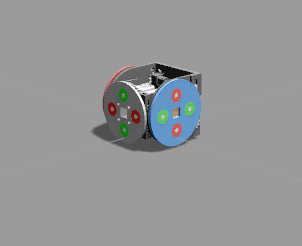
\includegraphics[height=\picHeight]{driver1.png} %&
            %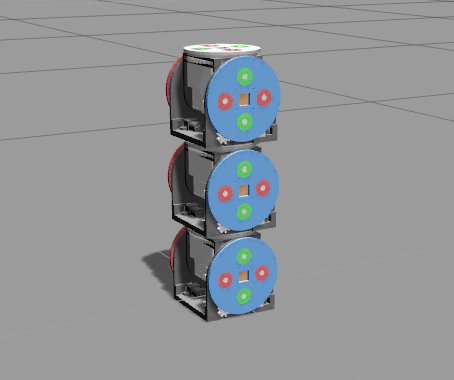
\includegraphics[height=\picHeight]{leg3.png} &
            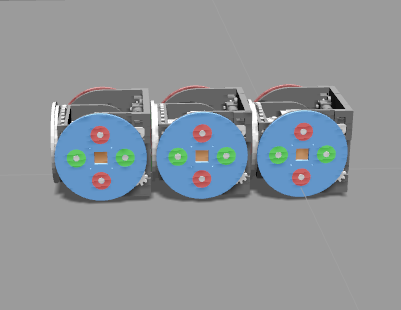
\includegraphics[height=\picHeight]{body3.png} %&
            %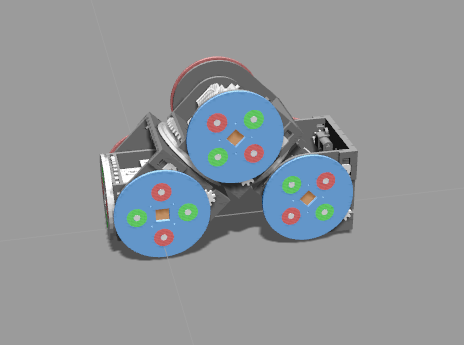
\includegraphics[height=\picHeight]{steer3.png} &
            %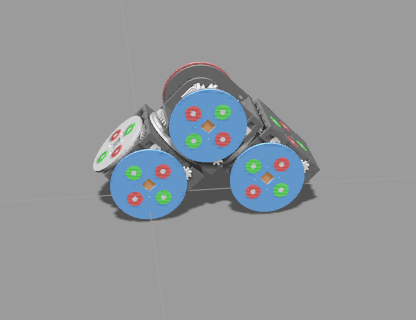
\includegraphics[height=\picHeight]{snake3.png} 
             \\ 
            %DRIVER1 & LEG3 & BODY3 & STEER3 & SNAKE3 
            CHAIN3
            \\ \hline
            %\pbox{20cm}{
            %\pbox{20cm}{\(Drive(v,t)\) \\ \(TiltMiddleUp()\)} \\
            %\pbox{20cm}{\(Step()\)} \\
            %\pbox{20cm}{\(HoldRigid()\)} \\
            %\pbox{20cm}{\(Steer(\theta)\) \\ \(DriveSideWheels(v,t)\)} \\ 
            %\pbox{20cm}{\(Wiggle()\) \\ \(AntiWiggle()\)} \\
            %
            \pbox{20cm}{\(Drive(v,t)\), \(SteeringPose()\), \(LegStep()\), \\ \(HoldRigid()\), \(Steer(\theta)\) }
            %}
            \\ \hline
        \end{tabular}
\end{document}








